\documentclass[11pt,a4paper]{article}

\usepackage[polish]{babel}
\usepackage{polski}
\usepackage[utf8]{inputenc}
\usepackage[T1]{fontenc}
\usepackage{graphicx}
\usepackage{color}
\usepackage{placeins}
\frenchspacing

\newcommand{\todo}[1]{\colorbox{yellow}{#1}}

\begin{document}

\title{Automatyczna klasyfikacja i ekstrakcja tematu krótkich notatek w języku polskim}
\author{Paweł Obrok\\pod kierunkiem dr. Michała Korzyckiego}

\maketitle
\pagebreak

\tableofcontents
\pagebreak

\section{Wstęp}
\section{Podstawy teoretyczne}
\section{Procedura badawcza}
\section{Opis danych}
\section{Wyniki i analiza}

Niniejszy rozdział zawiera porównanie różnych aspektów działania algorytmów LDA
i LSI. Na jego końcu znajdują się wnioski jakie można wyciągnąć z zebranych
danych.

\subsection{Tematy}

\subsection{Czas działania}

\subsection{Metryki z nadzorem}

\subsubsection{Ranking dokumentów}

Wykresy \ref{ranks_stemming_comparison}, \ref{ranks_no_stemming_comparison}
przedstawiają sumę kwadratów ranków dokumentów z wzorca przygotowanego ręcznie
dla danego zapytania w wynikach działania odpowiednio algorytmów LDA i LSI dla
różnej liczby tematów.

\begin{figure}
\caption{Suma kwadratów ranków dokumentów ze wzorca dla testowego zapytania (z wykorzystanie stemmingu)}
\label{ranks_stemming_comparison}
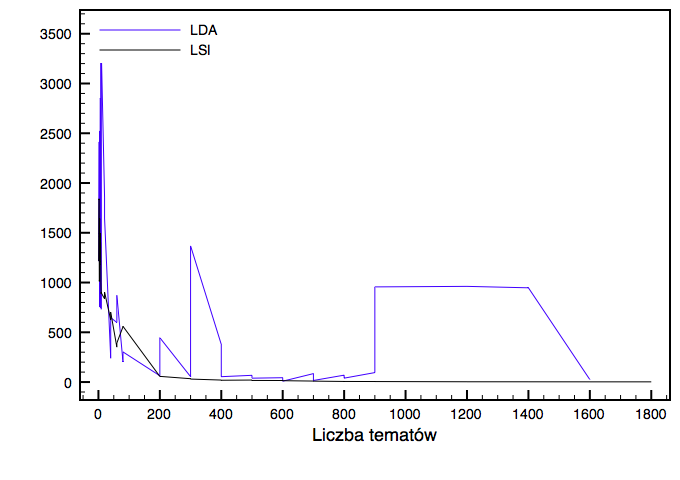
\includegraphics[width=\linewidth]{gfx/ranks_stemming.png}
\end{figure}

\begin{figure}
\caption{Suma kwadratów ranków dokumentów ze wzorca dla testowego zapytania (bez wykorzystania stemmingu)}
\label{ranks_no_stemming_comparison}
\todo{Wykres bez stemmingu}
\end{figure}

\FloatBarrier

\subsection{Krzywe ROC}

Krzywa ROC (Receiver Operation Characteristic) to wykres przedstawiający dla
danego klasyfikatora stosunek odsetka poprawnie odnalezionych dokumentów wśród
wszystkich dokumentów, które miały zostać odnalezione do odsetka odrzuconych
dokumentów wśród wszystkich dokumentów, które miały zostać odrzucone w miarę
zmiany progu detekcji. W tym wypadku ten zmienny próg to po prostu liczba $n$ -
pierwszych $n$ dokumentów jest traktowane jako odnalezione, a pozostałe jako
odrzucone.

Poniższe wykresy przedstawiają krzywe ROC dla algorytmów LDA i LSI dla różnych
liczb tematów.

\todo{Wykresy bez stemmingu - 20, 100, 300}
\todo{Wykresy ze stemmingiem - 20, 100, 300}

\subsection{Metryki bez nadzoru}

\subsection{Wnioski}

\section{Podsumowanie}

\enddocument
